%======================================================================%
% Filename: article.tex
% Project: Insight Journal Article, Alternative Memory Models for ITK images
% Author: Dan Mueller - dan.muel[at]gmail.com, dan.mueller[at]philips.com
% Date: $Date$
% Revision: $Revision$
%----------------------------------------------------------------------%
% Description:
% This artcile is for the Insight Journal.
% It describes alternative memory models for ITK images.
%======================================================================%
\documentclass{InsightArticle}

\usepackage{amsfonts}                 %Maths fonts
\usepackage{amssymb}                  %Maths symbols
\usepackage{listing}                  %Used for list of listings
\usepackage{listings}                 %List program code source
\usepackage{subfigure}                %For subfigures
\usepackage{color}                    %Allow color
\usepackage{fancyhdr}                 %Use headers and footers
\usepackage{graphicx}                 %Graphics
\usepackage{ccaption}
\usepackage[dvipdfm=true,
            bookmarks=true,
            bookmarksopen=true,
            bookmarksopenlevel=2,
            bookmarksnumbered=true,
            backref=section,
            colorlinks=true,
            linkcolor={blue},
            citecolor={blue},
            urlcolor={blue}]{hyperref}

%Allow code listings
%====================================================================
% Filename: listcode.tex
% Author: Daniel Mueller [d.mueller@qut.edu.au]
%--------------------------------------------------------------------
% Description: 
% Encapulates commands to list source code using the listings package.
% Also loads the [Shading]OpenGL language.
%--------------------------------------------------------------------
% Notes:
% - The listings package does not integrate well with the memoir class...
%	It may be necessary to delete the *.lol (local listing file) if an error
%   occurs during compilation.
%====================================================================              

%--------------------------------------------------------------------
% Define useful colours
\definecolor{listcomment}{rgb}{0.0,0.5,0.0}
\definecolor{listkeyword}{rgb}{0.0,0.0,0.5}
\definecolor{listnumbers}{gray}{0.65}
\definecolor{listlightgray}{gray}{0.955}
\definecolor{listwhite}{gray}{1.0}

%--------------------------------------------------------------------
% Configure C# listings
\newcommand{\listcsharp}
{
\lstset{frame = tb,
        framerule = 0.25pt,
        float,
        fontadjust,
        backgroundcolor={\color{listlightgray}},
        basicstyle = {\ttfamily\footnotesize},
        keywordstyle = {\ttfamily\color{listkeyword}\textbf},
        identifierstyle = {\ttfamily},
        commentstyle = {\ttfamily\color{listcomment}\textit},
        stringstyle = {\ttfamily},
        showstringspaces = false,
        showtabs = false,
        numbers = left,
        numbersep = 6pt,
        numberstyle={\ttfamily\color{listnumbers}},
        tabsize = 2,
        language=[Sharp]C,
        floatplacement=!h
        }
}

%--------------------------------------------------------------------
% Configure C# snippets
\newcommand{\listcsharpsnip}
{
\lstset{frame = none,
        framerule = 0.0pt,
        float,
        fontadjust,
        backgroundcolor={\color{listlightgray}},
        basicstyle = {\ttfamily\footnotesize},
        keywordstyle = {\ttfamily\color{listkeyword}\textbf},
        identifierstyle = {\ttfamily},
        commentstyle = {\ttfamily\color{listcomment}\textit},
        stringstyle = {\ttfamily},
        showstringspaces = false,
        showtabs = false,
        numbers = left,
        numbersep = 6pt,
        numberstyle={\ttfamily\color{listnumbers}},
        tabsize = 2,
        language=[Sharp]C,
        floatplacement=!h
        }
}

%--------------------------------------------------------------------
% Configure C++ snippets
\newcommand{\listcpluspluspsnip}
{
\lstset{frame = none,
        framerule = 0.0pt,
        float,
        fontadjust,
        backgroundcolor={\color{listlightgray}},
        basicstyle = {\ttfamily\footnotesize},
        keywordstyle = {\ttfamily\color{listkeyword}\textbf},
        identifierstyle = {\ttfamily},
        commentstyle = {\ttfamily\color{listcomment}\textit},
        stringstyle = {\ttfamily},
        showstringspaces = false,
        showtabs = false,
        numbers = left,
        numbersep = 6pt,
        numberstyle={\ttfamily\color{listnumbers}},
        tabsize = 2,
        gobble = 4,
        language=[ISO]C++,
        floatplacement=!h
        }
}

%--------------------------------------------------------------------
% Configure console snippets
\newcommand{\listconsolesnip}
{
\lstset{frame = none,
        framerule = 0.0pt,
        float,
        fontadjust,
        backgroundcolor={\color{listlightgray}},
        basicstyle = {\ttfamily\footnotesize},
        keywordstyle = {\ttfamily},
        identifierstyle = {\ttfamily},
        commentstyle = {\ttfamily},
        stringstyle = {\ttfamily},
        showstringspaces = false,
        showtabs = false,
        numbers = none,        
        tabsize = 2,
        floatplacement=!h
        }
}

%--------------------------------------------------------------------
% Configure python listings
\newcommand{\listpython}
{
\lstset{frame = tb,
        framerule = 0.25pt,
        float,
        fontadjust,
        backgroundcolor={\color{listlightgray}},
        basicstyle = {\ttfamily\footnotesize},
        keywordstyle = {\ttfamily\color{listkeyword}\textbf},
        identifierstyle = {\ttfamily},
        commentstyle = {\ttfamily\color{listcomment}\textit},
        stringstyle = {\ttfamily},
        showstringspaces = false,
        showtabs = false,
        numbers = left,
        numbersep = 6pt,
        numberstyle={\ttfamily\color{listnumbers}},
        tabsize = 2,
        language=Python,
        floatplacement=!h
        }
}

\newcommand{\listpythonsmall}
{
\lstset{frame = tb,
        framerule = 0.25pt,
        float,
        fontadjust,
        backgroundcolor={\color{listlightgray}},
        basicstyle = {\ttfamily\scriptsize},
        keywordstyle = {\ttfamily\color{listkeyword}\textbf},
        identifierstyle = {\ttfamily},
        commentstyle = {\ttfamily\color{listcomment}\textit},
        stringstyle = {\ttfamily},
        showstringspaces = false,
        showtabs = false,
        numbers = left,
        numbersep = 6pt,
        numberstyle={\ttfamily\color{listnumbers}},
        tabsize = 2,
        language=Python,
        floatplacement=!h
        }
}

%--------------------------------------------------------------------
% Configure python snippets
\newcommand{\listpythonsnip}
{
\lstset{frame = none,
        framerule = 0pt,
        float,
        fontadjust,
        backgroundcolor={\color{listlightgray}},
        basicstyle = {\ttfamily\footnotesize},
        keywordstyle = {\ttfamily\color{listkeyword}\textbf},
        identifierstyle = {\ttfamily},
        commentstyle = {\ttfamily\color{listcomment}\textit},
        stringstyle = {\ttfamily},
        showstringspaces = false,
        showtabs = false,
        numbers = left,
        numbersep = 6pt,
        numberstyle={\ttfamily\color{listnumbers}},
        tabsize = 2,
        language=Python,
        floatplacement=tb
        }
}

%--------------------------------------------------------------------
% Configure make listings
\newcommand{\listmake}
{
\lstset{frame = tb,
        framerule = 0.25pt,
        float,
        fontadjust,
        backgroundcolor={\color{listlightgray}},
        basicstyle = {\ttfamily\footnotesize},
        keywordstyle = {\ttfamily\color{listkeyword}\textbf},
        identifierstyle = {\ttfamily},
        commentstyle = {\ttfamily\color{listcomment}\textit},
        stringstyle = {\ttfamily},
        showstringspaces = false,
        showtabs = false,
        numbers = left,
        numbersep = 6pt,
        numberstyle={\ttfamily\color{listnumbers}},
        tabsize = 2,
        language=make,
        floatplacement=!h
        }
}

%--------------------------------------------------------------------
% Configure GLSL listings
\newcommand{\listglsl}
{
\lstset{frame = tb,
        framerule = 0.25pt,
        float,
        fontadjust,
        backgroundcolor={\color{listlightgray}},
        basicstyle = {\ttfamily\footnotesize},
        keywordstyle = {\ttfamily\color{listkeyword}\textbf},
        identifierstyle = {\ttfamily},
        commentstyle = {\ttfamily\color{listcomment}\textit},
        stringstyle = {\ttfamily},
        showstringspaces = false,
        showtabs = false,
        numbers = left,
        numbersep = 6pt,
        numberstyle={\ttfamily\color{listnumbers}},
        tabsize = 2,
        language=[Shading]OpenGL,
        floatplacement=!h
        }
}

%--------------------------------------------------------------------
% Configure GLSL snippets
\newcommand{\listglslsnip}
{
\lstset{frame = none,
        framerule = 0pt,
        float,
        fontadjust,
        backgroundcolor={\color{listlightgray}},
        basicstyle = {\ttfamily\footnotesize},
        keywordstyle = {\ttfamily\color{listkeyword}\textbf},
        identifierstyle = {\ttfamily},
        commentstyle = {\ttfamily\color{listcomment}\textit},
        stringstyle = {\ttfamily},
        showstringspaces = false,
        showtabs = false,
        numbers = left,
        numbersep = 6pt,
        numberstyle={\ttfamily\color{listnumbers}},
        tabsize = 2,
        language=[Shading]OpenGL,
        floatplacement=!h
        }}

%--------------------------------------------------------------------
% Define the OpenGL Shading language keywords, comments, etc...
\lstdefinelanguage[Shading]{OpenGL}%
{%
    morekeywords=   {%
                    attribute,%
                    const,%
                    uniform,%
                    varying,%
                    break,%
                    continue,%
                    do,%
                    for,%
                    while,%
                    if,%
                    else,%
                    in,%
                    out,%
                    inout,%
                    true,%
                    false,%
                    discard,%
                    return,%
                    float,%
                    int,%
                    void,%
                    bool,%
                    mat2,%
                    mat3,%
                    mat4,%
                    vec2,
                    vec3,%
                    vec4,%
                    ivec2,%
                    ivec3,%
                    ivec4,%
                    bvec2,%
                    bvec3,%
                    bvec4,%
                    sampler1D,%
                    sampler2D,%
                    sampler3D,%
                    samplerCube,%
                    sampler1DShadow,%
                    sampler2DShadow,%
                    struct,%
                    radians,%
                    degrees,%
                    sin,%
                    cos,%
                    tan,%
                    asin,%
                    acos,%
                    atan,%
                    pow,%
                    exp2,%
                    log2,%
                    sqrt,%
                    inversesqrt,%
                    abs,%
                    sign,%
                    floor,%
                    ceil,%
                    fract,%
                    mod,%
                    min,%
                    max,%
                    clamp,%
                    mix,%
                    step,%
                    smoothstep,%
                    length,%
                    distance,%
                    dot,%
                    cross,%
                    normalize,%
                    transform,%
                    faceforward,%
                    reflect,%
                    matrixCompMult,%
                    lessThan,%
                    lessThanEqual,%
                    greaterThan,%
                    greaterThanEqual,%
                    equal,%
                    notEqual,%
                    any,%
                    all,%
                    not,%
                    texture1D,%
                    texture1DProj,%
                    texture1DProjLod,%
                    texture2D,%
                    texture2DProj,%
                    texture2DProjLod,%
                    texture3D,%
                    texture3DProj,%
                    texture3DProjLod,%
                    textureCube,%
                    textureCubeLod,%
                    shadow1D,%
                    shadow1DProj,%
                    shadow1DLod,%
                    shadow1DProjLod,%
                    shadow2D,%
                    shadow2DProj,%
                    shadow2DLod,%
                    shadow2DProjLod,%
                    dFdx,%
                    dFdy,%
                    fwidth,%
                    noise1,%
                    noise2,%
                    noise3,%
                    noise4},%
    morekeywords={%
                    gl_Position,%
                    gl_PointSize,%
                    gl_ClipVertex,%
                    gl_FragCoord,%
                    gl_FrontFacing,%
                    gl_FragColor,%
                    gl_FragDepth,%
                    gl_Color,%
                    gl_SecondaryColor,%
                    gl_Normal,%
                    gl_Vertex,%
                    gl_MultiTexCoord0,%
                    gl_MultiTexCoord1,%
                    gl_MultiTexCoord2,%
                    gl_MultiTexCoord3,%
                    gl_MultiTexCoord4,%
                    gl_MultiTexCoord5,%
                    gl_MultiTexCoord6,%
                    gl_MultiTexCoord7,%
                    gl_FogCoord,%
                    gl_MaxLights,%
                    gl_MaxClipPlanes,%
                    gl_MaxTextureUnits,%
                    gl_MaxTextureCoordsARB,%
                    gl_MaxVertexAttributesGL2,%
                    gl_MaxVertexUniformFloatsGL2,%
                    gl_MaxVaryingFloatsGL2,%
                    gl_MaxVertexTextureUnitsGL2,%
                    gl_MaxFragmentTextureUnitsGL2,%
                    gl_MaxFragmentUniformFloatsGL2,%
                    gl_ModelViewMatrix,%
                    gl_ProjectionMatrix,%
                    gl_ModelViewProjectionMatrix,%
                    gl_NormalMatrix,%
                    gl_TextureMatrix,%
                    gl_NormalScale,%
                    gl_DepthRange,%
                    gl_ClipPlane,%
                    gl_Point,%
                    gl_FrontMaterial,%
                    gl_BackMaterial,%
                    gl_LightSource,%
                    gl_LightModel,%
                    gl_FrontLightModelProduct,%
                    gl_BackLightModelProduct,%
                    gl_FrontLightProduct,%
                    gl_LightProducts,%
                    gl_TextureEnvColor,%
                    gl_EyePlaneS,%
                    gl_EyePlaneT,%
                    gl_EyePlaneR,%
                    gl_EyePlaneQ,%
                    gl_ObjectPlaneS,%
                    gl_ObjectPlaneT,%
                    gl_ObjectPlaneR,%
                    gl_ObjectPlaneQ,%
                    gl_Fog,%
                    gl_FrontColor,%
                    gl_BackColor,%
                    gl_FrontSecondaryColor,%
                    gl_BackSecondaryColor,%
                    gl_TexCoord,%
                    gl_FogFragCoord,%
                    gl_Color,%
                    gl_SecondaryColor,%
                    gl_TexCoord,%
                    gl_FogFragCoord},%                   
    sensitive,%
    morecomment=[s]{/*}{*/},%
    morecomment=[l]//,%
    morestring=[b]"
    }[keywords,comments,strings]%

%--------------------------------------------------------------------
% Load [Shading]OpenGL for use with the listings package 
\lstloadlanguages{[Shading]OpenGL}
                 

%======================================================================%
%                   F r o n t   M a t t e r                            % 
%======================================================================%

\title{Alternative Memory Models for ITK Images}
 
% NOTE: This is the last number of the "handle" URL that 
% The Insight Journal assigns to your paper as part of the
% submission process. Please replace the number "1338" with
% the actual handle number that you get assigned.
\newcommand{\IJhandlerIDnumber}{3068}

% Increment the release number whenever significant changes are made.
% The author and/or editor can define 'significant' however they like.
\release{1.02}

% At minimum, give your name and an email address.
\author{Dan Mueller$^{1}$}
\authoraddress{$^{1}$Philips Informatics Infrastructure (PII), Philips Healthcare, Best, Netherlands}

\begin{document}

% Add hyperlink to the web location and license of the paper.
% The argument of this command is the handler identifier given
% by the Insight Journal to this paper.
\IJhandlefooter{\IJhandlerIDnumber}

\maketitle

\ifhtml
\chapter*{Front Matter\label{front}}
\fi

%======================================================================%
%                       A b s t r a c t                                % 
%======================================================================%

% The abstract should be a paragraph or two long, and describe the
% scope of the document.
\begin{abstract}
\noindent
By default ITK images employ a contiguous memory model.
This means pixel elements are stored in a single 1-D array,
where each element is adjacent in memory to the previous element.
However in some situations a contiguous memory model is not desirable.
%
This document describes three alternative memory models: slice contiguous,
sparse, and single-bit binary images.
%
A slice contiguous image is a three-dimensional image whereby each
slice is stored in a contiguous 1-D array, but the slices are not
necessarily adjacent in memory.
Slice contiguous images are well suited for interoperability with
applications representing images using DICOM.
%
A sparse image is an $n$-dimensional image in which each pixel is stored
in a hash table data structure.
This memory model is well suited for images with very large dimensions,
but few pixels that are actually relevant.
%
A single-bit binary image is an $n$-dimensional image that internally
stores a boolean as a single-bit, rather than the typical eight-bits.
Single-bit images allow very compact representations for on-off binary masks.
%
Source code, tests, and examples are provided to allow easy reproduction
and use.

\end{abstract}

\IJhandlenote{\IJhandlerIDnumber}

%======================================================================%
%                     M a i n   M a t t e r                            % 
%======================================================================%
\tableofcontents

%----------------------------------------------------------------------%
% Section
%----------------------------------------------------------------------%
\section{Introduction}

ITK images currently employ an implicit contiguous memory model.
By implicit we mean that the memory model is tightly coupled with many other
classes within the toolkit.
By contiguous we mean that pixel elements are stored as a 1-D array,
where each element is adjacent in memory to the previous element.
This underlying pixel array is not hidden behind a layer of abstraction but
can be easily accessed using for example \code{itk::Image::GetBufferPointer()}.

Performing a quick \code{grep} over the codebase reveals numerous classes
which directly access the image pixel array in this manner.
Such tight coupling makes it difficult to abstract away the underlying memory
model used by the image to store the pixel data.
Some of the important classes which directly access the pixel array using
\code{itk::Image::GetBufferPointer()} include:
image iterators, image adpaters, image file readers/writers, and the VTK image export filter.
A number of other minor classes also directly access the pixel array, such as:
octree, watershed segmenter, BSpline deformable transform, 
optimized Mattes mutual information metric, etc.

The existence of classes which directly access the pixel array,
as well as ITK's strict backward compatibility policy,
makes it difficult --- but not impossible --- to introduce images with alternative memory models.
This paper uses the same approach employed by \code{itk::VectorImage} to realize three new
memory models for ITK images. The new image types do not require changes to the toolkit,
and function with a majority of the existing filters and iterators.
However they are only interoperable with classes which do not directly access the pixel array.
For example it is not possible to use image IO, export to VTK, or
use the optimized registration framework with the proposed images.%
%
\vspace{-1mm}
\begin{figure}[!htb]
    \centering
    \subfigure[Contiguous Memory Model]{
    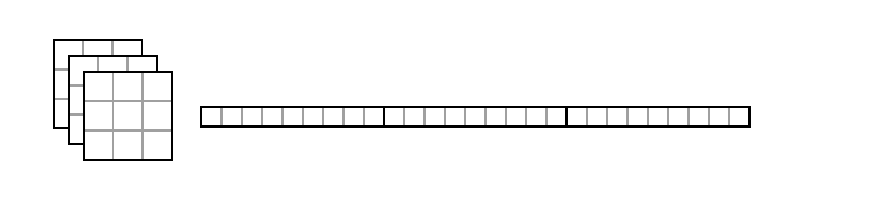
\includegraphics[width=0.85\textwidth]{contiguous-memory-model.eps}}
    \subfigure[Slice Contiguous Memory Model]{
    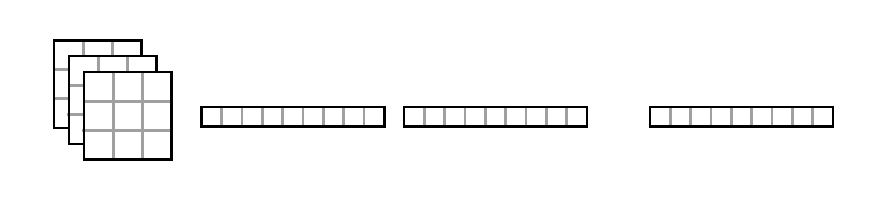
\includegraphics[width=0.85\textwidth]{slice-contiguous-memory-model.eps}}   
    \caption{\label{fig:Introduction:Models}%
    Contiguous and slice contiguous memory models.}
\end{figure}
%
%----------------------------------------------------------------------%
% Section
%----------------------------------------------------------------------%
%\newpage%
\vspace{-7mm}
\section{Proposed Image Memory Models}

\subsection{Slice Contiguous Images}
A slice contiguous image is implicitly three-dimensional.
Each slice is stored in a contiguous 1-D array,
but the slices are not necessarily adjacent in memory.
This representation is shown in \figurename~\ref{fig:Introduction:Models}.
The new \code{itk::SliceContiguousImage} may be useful 
for interoperability with existing code representing images using a
slice contiguous memory model.
This scenario is common for third party applications using DICOM.

This paper proposes an implementation for an image with such a memory model.
This is realized by creating a new image class with custom
pixel and neighborhood accessor functions;
similar to \code{itk::VectorImage}.
The pixel and neighborhood accessor functions provide a layer of
indirection for iterators to access the image pixel data.
Given the incoming offset for a contiguous memory model,
the new accessors compute the index of the slice containing the pixel
and the offset within that slice.
The new image class is templated over the pixel type;
it is not templated over the number of dimensions because it is always three.

One important different between \code{itk::Image} and \code{itk::SliceContiguousImage}
is that for the later \code{GetBufferPointer()} always returns \code{NULL}
ie. the pixel buffer makes no sense.
Ideally this method would not even exist for slice contiguous images,
but unfortunately too many other classes assume its existence.

A slice contiguous image is created in a very similar fashion to a ``normal'' image:
\listcpluspluspsnip
\lstinputlisting[float,label=lst:Slice1,linerange={39-39,42-42,44-44,78-87}]
                 {../Testing/SliceContiguousImageTest01.cxx}

An additional step requires the pixel container to be configured
with a list of slice pointers:
\listcpluspluspsnip
\lstinputlisting[float,label=lst:Slice2,linerange={89-98}]
                 {../Testing/SliceContiguousImageTest01.cxx}

The slice contiguous image can now be used like any other image:
\listcpluspluspsnip
\lstinputlisting[float,label=lst:Slice3,linerange={140-146}]
                 {../Testing/SliceContiguousImageTest01.cxx}

\vspace{-10mm}
\subsection{Sparse Images}
A sparse image is an $n$-dimensional image in which each pixel is stored
in a hash table data structure.
Each time a pixel is set, a new offset-value pair is added to the hash table.
Such a memory model means that little or no memory is allocated when the
image is created, but the memory footprint grows as more and more pixels
are set.
This memory model is well suited for images with very large dimensions,
but few pixels which are actually relevant.
It should be noted that (at least for the moment) filters using images
with this memory model must be single threaded.

A sparse image can be created in the typical fashion:
\listcpluspluspsnip
\lstinputlisting[float,label=lst:Sparse1,linerange={39-42,47-48,50-57}]
                 {../Testing/SparseImageTest01.cxx}

A sparse image requires a ``background'' value to be specified for
undefined pixels:
\listcpluspluspsnip
\lstinputlisting[float,label=lst:Sparse2,linerange={170-170}]
                 {../Testing/SparseImageTest01.cxx}

Pixels can be retrieved or set directly (using \code{Get}/\code{SetPixel})
or via an iterator:
\listcpluspluspsnip
\lstinputlisting[float,label=lst:Sparse3,linerange={170-172,174-176}]
                 {../Testing/SparseImageTest01.cxx}
\vspace{-10mm}
\subsection{Single-bit Binary Images}
It is very common in image processing to create mask images which
indicate regions which are ``on'' or ``off''.
Currently the smallest pixel element available in ITK for representing such
images is \code{unsigned char} which is stored in a single byte (eight-bits).
Even though a \code{bool} value can only represent \code{0} or \code{1},
it too is stored in a single byte (you can check this by writing out \code{sizeof(bool)}).

Single-bit binary images internally represent each pixel as a single-bit.
As such the memory footprint for on-off masks can be lowered by (nearly) a factor of eight.
Similar to slice contiguous images, single-bit binary images provide custom pixel
accessor functions which convert the incoming offset to the relevant bit mask for the
underlying data storage.
Unlike slice contiguous images, single-bit binary images fit slightly better within the
existing ITK framework so \code{GetBufferPointer()} makes sense in this context.

A single-bit binary image can be created in the typical fashion:
\listcpluspluspsnip
\lstinputlisting[float,label=lst:Binary1,linerange={39-42,48-58}]
                 {../Testing/SingleBitBinaryImageTest01.cxx}

The bits are stored in blocks of 32, so the above code will actually
allocate a buffer with size $96 \times 96$.
As with all the presented image class, the binary image can be used with
any iterator and/or filter
which does not directly access the pixel buffer via \code{GetBufferPointer()}.

%----------------------------------------------------------------------%
% Section
%----------------------------------------------------------------------%
\section{Performance}
Although the memory models presented above may be advantageous for
reducing memory usage in certain scenarios,
they have a performance penalty.
Accessing pixels stored in a contiguous array can be highly efficient,
whereas the three new images require additional computation each time a pixel is accessed.
%
This section provides a simple analysis of the performance for each
of the proposed images.

The performance test measured four properties:
(1) time to allocate the buffer,
(2) time to fill the buffer,
(3) time to set all pixels using an iterator, and
(4) time to get all pixels using an iterator.
Each test was run on a $256 \times 256 \times 256$ image,
executed on my notebook (Intel Core 2 Duo, T7250 @ 2GHz, 3GB RAM, Windows Vista SP1 32-bit)
a total of 5 times with mean times (in seconds) reported in the table below.

As can be seen, all the images have similar values for buffer allocation and 
getting pixels using an iterator.
The sparse image was the fastest for filling the buffer
because no memory is actually set at this moment, only a single ``background'' value.
However it was also the slowest (by quite a margin) for setting pixels using an iterator,
because each pixel being set must be added to the hash table.
The single-bit binary image was comparably fast for filling the buffer because
the pixels are set in groups of 32-bits, rather than individual elements.%
%
%Contiguous Allocate: 1.2207e-005
%Contiguous FillBuffer: 0.0460442
%Contiguous IterateSet: 0.0465508
%Contiguous IterateGet: 0.0192841
%SliceContiguous Allocate: 0.00140305
%SliceContiguous FillBuffer: 0.0539986
%SliceContiguous IterateSet: 0.131505
%SliceContiguous IterateGet: 0.0205986
%Sparse Allocate: 2.28882e-006
%Sparse FillBuffer: 1.52588e-006
%Sparse IterateSet: 6.52589
%Sparse IterateGet: 0.0190674
%Binary Allocate: 1.98364e-005
%Binary FillBuffer: 0.00196152
%Binary IterateSet: 0.0708679
%Binary IterateGet: 0.0198059
%
\begin{table}[!htb]
\begin{center}
\begin{tabular}{l|llll}
    \hline
    Image Type & Allocation & FillBuffer & Iterate Set & Iterate Get \\
    \hline
    \hline
	  Contiguous & $< 0.01$ & $0.05$ & $0.05$ & $0.02$ \\
	  Slice Contiguous & $0.01$ & $0.05$ & $0.13$ & $0.02$ \\
	  Sparse & $< 0.01$ & $< 0.01$ & $6.53$ & $0.02$ \\
	  Binary & $< 0.01$ & $< 0.01$ & $0.07$ & $0.02$ \\
    \hline
\end{tabular}
\caption[Performance results (in seconds)]
{Performance timings in seconds for a $256 \times 256 \times 256$ image.}
\label{table:performance}
\end{center}
\end{table}

%----------------------------------------------------------------------%
% Section
%----------------------------------------------------------------------%
\section{Conclusion}
This submission proposed three images with alternative memory models:
slice contiguous, sparse, and single-bit binary images.
For the moment there is no IO support for any of the proposed images,
however it might be possible to provide such support in the future.
The proposed images should work seamlessly with most of the existing ITK filters
--- assuming they access the pixel data using iterators rather than
\code{GetBufferPointer()}.
These new images are just a few of the possible alternate memory models
and should provide a good guide for others wanting to develop their own.

%----------------------------------------------------------------------%
% Section
%----------------------------------------------------------------------%
\section{Acknowledgments}
Thanks to Karthik Krishnan (Kitware) and Glen Lehmann (Calgary Scientific)
for helpful discussions.

%======================================================================%
%                    B i b l i o g r a p h y                           % 
%======================================================================%
%\bibliographystyle{plain}
%\bibliography{article}

\end{document}